\documentclass{article}
\usepackage{graphicx} % Required for inserting images

\title{Notes on Oximeters}
\author{Arsh Arora}
\date{May 2023}

\begin{document}

\maketitle

\section{Introduction}
these are my notes on oximeters with a special emphasis on pulse oximeters written in order to study the working of them and later use them in a project which strongly revolves around them. This has been written in \LaTeX \, to ensure uniformity and global easiness to access.
\section{Oximetry}
Oximetery is defined as the determination of oxygen saturation of circulating arterial blood.
\begin{equation}
    Oxygen\:Saturation\:=\: \frac{[HbO_2]}{[HbO_2] + [Hb]}
\end{equation}
This saturation being a bio-constant, is an indications of the performance of the most important cardio-respiratory functions. It is maintained at a fairly constant value to within a few percent in an healthy organism. Oximetery is now a standard factor to consider for anaesthesiology and has significantly reduced anaesthesia related cardiac arrests. 
\subsection{In-vitro Oximetry}
When blood is withdrawn from the subject under anaerobic conditions and measurement for oxygen saturation is made at a later time in the laboratory, the procedure is referred to as in vitro oximetry.
\subsubsection{Transmission Oximetry}
Measurement of the degree of oxygen saturation of the blood can be made by spectrophotometric method. In spectrophotometry, the concentrations of substances held in solution are measured by determining the relative light attenuations that the light absorbing substances cause at each of several wavelengths. 
\begin{equation}
    I\: = \: {I_O}^{-kCb}
\end{equation}
\begin{equation}
    Absorbance = kCb
\end{equation}
We can study the spectral transmission characteristics of oxyhaemoglobin and reduced haemoglobin in the visible and infrared regions of spectrum in the graph below.
\begin{center}
    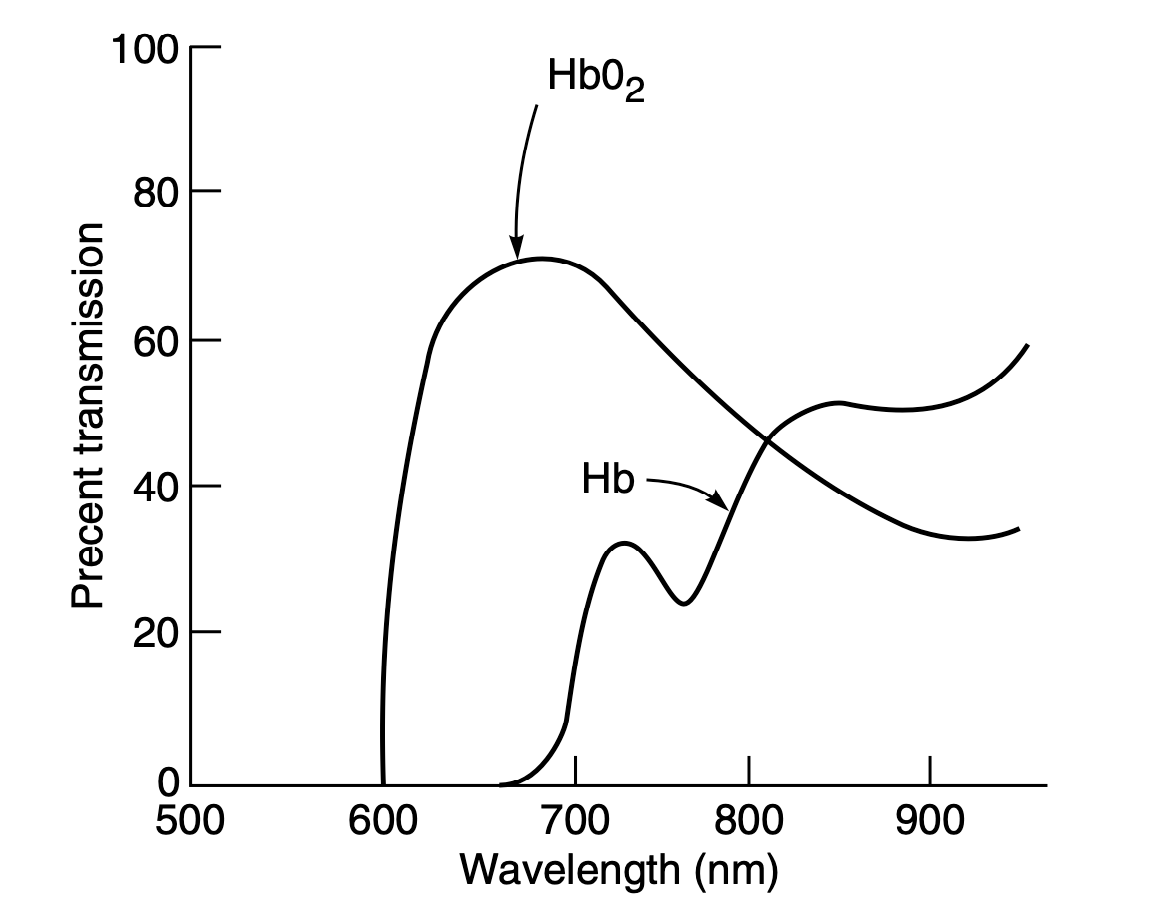
\includegraphics[scale=0.4]{Screenshot 2023-05-04 at 6.00.01 PM.png}
\end{center}
If the transmission which occur at 670nm and 820nm are taken in consideration, we can very clearly iron out the diffrerence between blood and find it saturation relatively.\\
\\
The Lambert-Beer law or the spectrophotometric technique applies only to haemolyzed blood, i.e. to blood in which the individual red cells have been destroyed and the pigments contained in the cells are homogeneously distributed in the whole solution. This is necessary to eliminate artefacts associated with multiple scattering of the measuring light from erythrocytes. 
\subsubsection{Reflective Oximetry}
Reflection oximetry is based on the scattering of light by the erythrocytes. For the light scattered from the unhaemolyzed blood sample, oxygen saturation is given by:
\begin{equation}
    Oxygen\, Saturation\: = \: \frac{I_r (\lambda_2)}{I_r (\lambda_1)} + b_r
\end{equation}
Polanyi and Hehir (1960) showed experimentally that a linear relationship exists between $I_r(\lambda2)/I_r(\lambda1)$ and oxygen saturation.\\
They computed the relationship as follows:
\begin{equation}
    Oxygen\: Saturation \: = \: 1.13 - 0.28 \cdot \frac{I_r (805)}{I_r (650)}
\end{equation}
\newpage
\subsection{In-Vivo Oximetry}
In vivo oximetry measures the oxygen saturation of blood while the blood is flowing through the vascular system or it may be flowing through a cuvette directly connected with the circulatory system by means of a catheter. The blood in this case is unhaemolyzed.
\begin{center}
    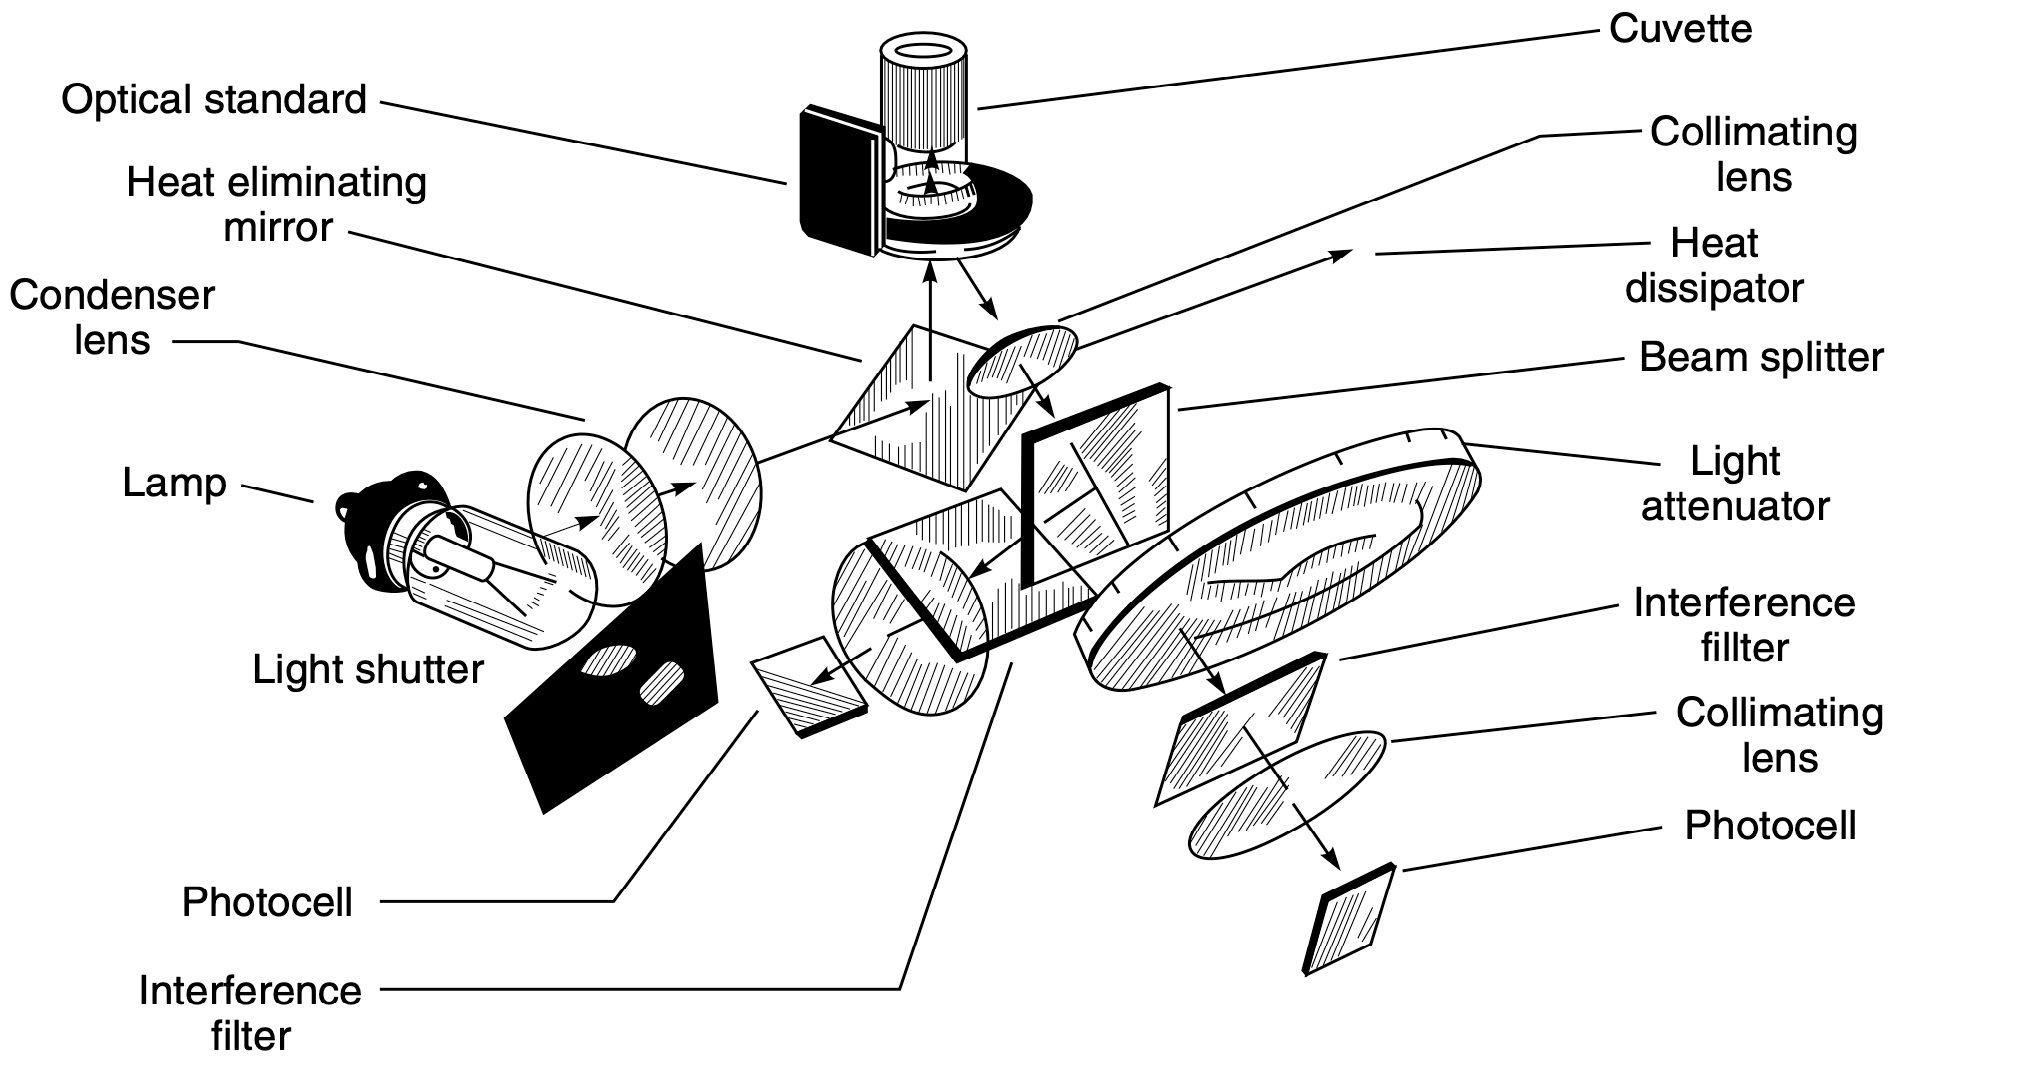
\includegraphics[scale=0.3]{Screenshot 2023-05-04 at 6.54.44 PM.png}
\end{center}
\section{Pulse Oximeter}
Pulse oximetry is a concept owed only to the theory that determination can be done using two wavelengths, provided the measurements are made on the pulsatile part of the wave- form. The two wavelengths assume that only two absorbers are present; namely oxyhaemoglobin ($HbO_2$) and reduced haemoglobin (Hb).
\begin{enumerate}
    \item Light passing through the ear or finger will be absorbed by skin pigments, tissue, cartilage, bone, arterial blood, venous blood.
    \item The absorbance are additive and obey Beer-Lamber law:
    \begin{equation}
        A\:=\: -logT\:=\: log \frac{I_0}{I} = \epsilon D C
    \end{equation}
    where Io and I are incident and transmitted light intensities, $\epsilon$ is the extinction coefficient, D is the depth of the absorbing layer and C is concentration.
    \item Most of the absorbances are fixed and do notchange with time.
\end{enumerate}
Therefore, only measuring the changing signal, measures only the absorbance due to arterial blood and makes possible the determination of arterial oxygen saturation (SaO2). \\
\\
This has two LEDs (light emitting diodes), one that transmits infrared light at a wavelength of approximately 940 nm and the other transmitting light at approximately 660 nm. The absorption of these select wavelengths of light through living tissues is significantly different for oxygenated haemoglobin (HbO2) and reduced haemoglobin (Hb). The absorption of these selected wavelengths of light passing through living tissue is measured with a photosensor.
\begin{center}
    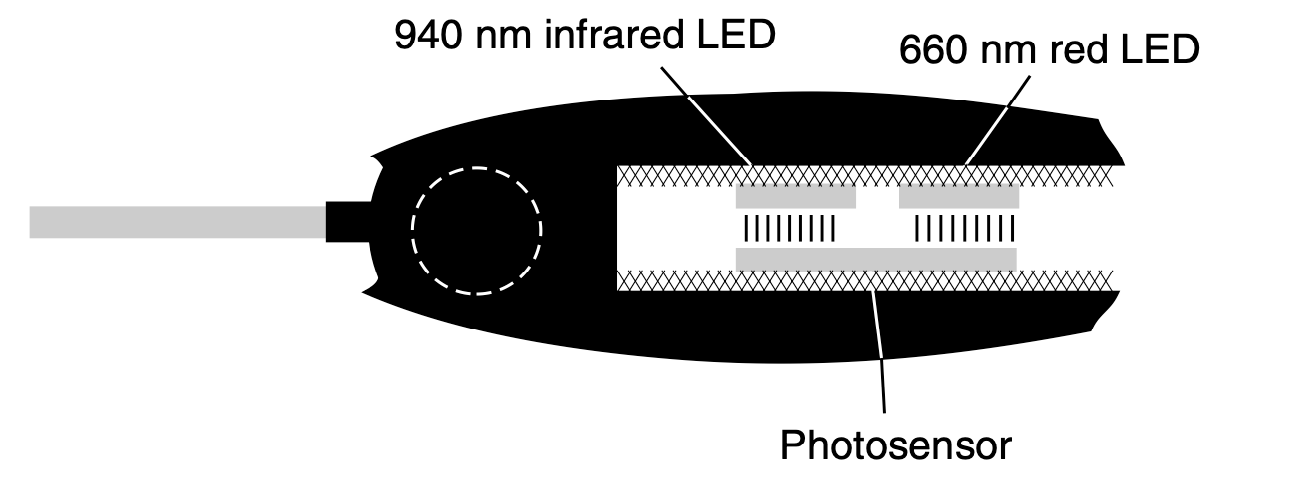
\includegraphics[scale=0.4]{Screenshot 2023-05-05 at 2.04.01 AM.png}
    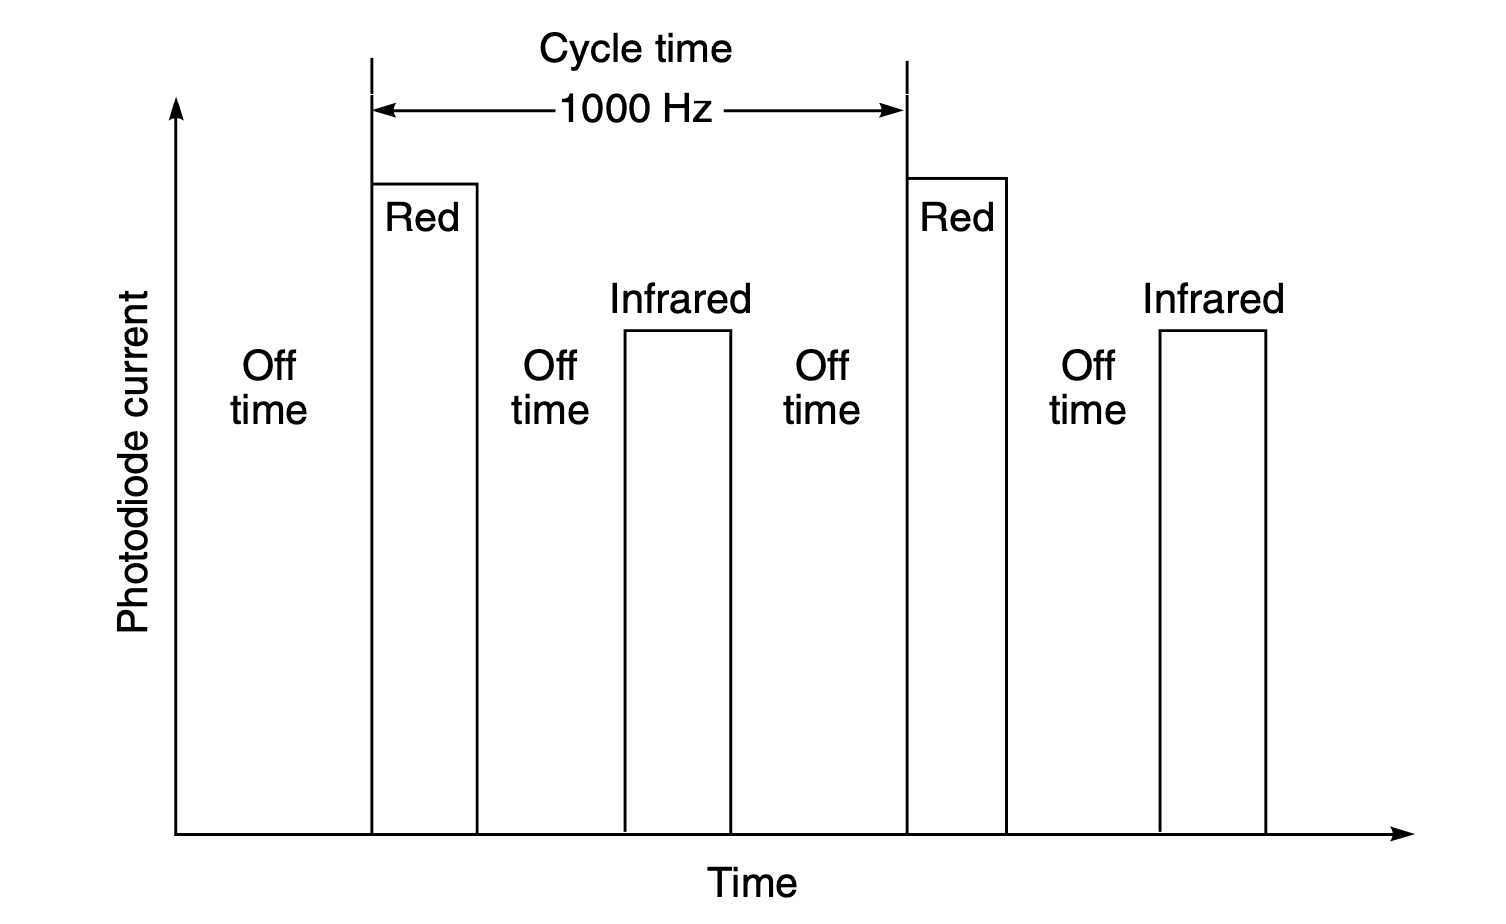
\includegraphics[scale=0.4]{Screenshot 2023-05-05 at 2.04.55 AM.png}
\end{center}
Oxygen saturation is estimated from the ratio (R) of pulse-added red absorbance at 660 nm to the pulse-added infrared absorbances at 940 nm.
\begin{equation}
    R \: = \: \frac{ac\, 600 / dc \, 660}{ac \, 940 / dc\, 940}
\end{equation}
The signal from the sensor is a current. The first amplifier stage is a current to voltage converter. The voltage signal then goes through the following circuits: amplifiers to further amplify the signal; noise filters to remove different kinds of interference, a demultiplexer to separate the interleaved red and infrared signals; bandpass filters to separate the low frequency (dc) component from the pulsatile, higher frequency (ac) component; and an analog–digital converter to convert the continuously varying signal to a digital representation.
\\
\begin{center}
    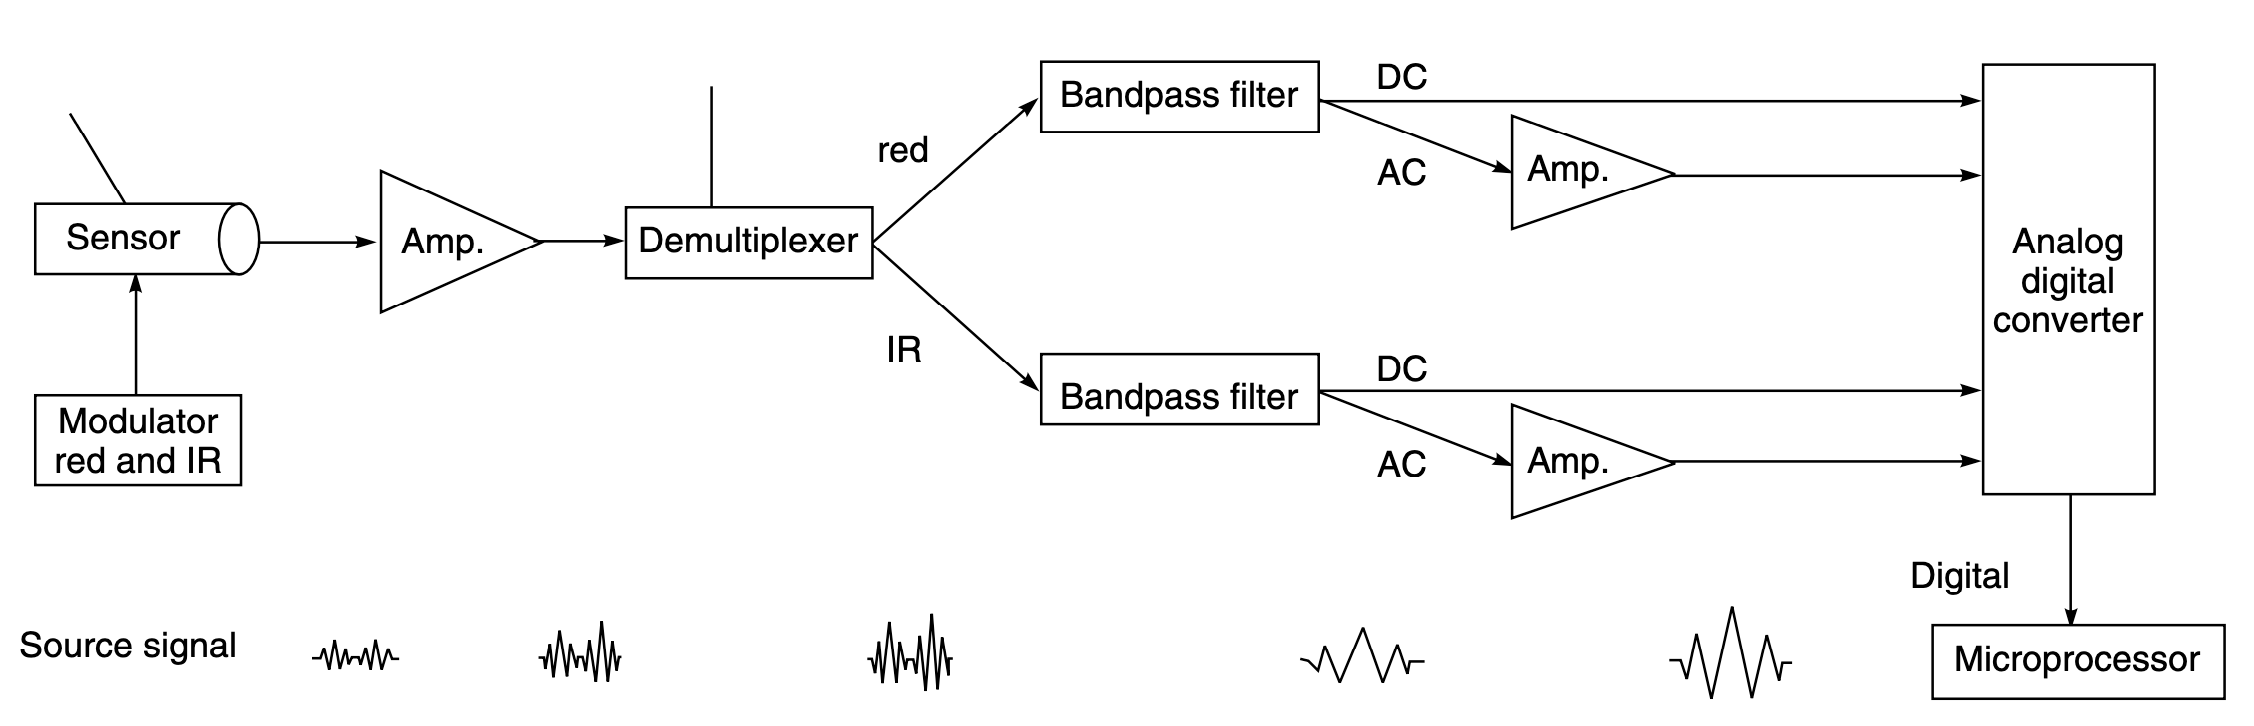
\includegraphics[scale=0.3]{Screenshot 2023-05-05 at 2.09.55 AM.png}
\end{center}

\textbf{Limitation of pusle oximeter} A limitation of the pulse oximeter is that ambient lights have been shown to interfere with the measurement. Therefore, covering the cuff with an opaque material is necessary to prevent such interference. Motion artifact is also a potential problem. This is because the information containing pulse activity is in the same frequency range as motion artifact.
\section{Skin reflectance oximeter}
For the measurement of oxygen saturation level of blood in localized areas of oxygen deprived tissues on the limbs, head and torso, a skin reflectance oximeter can be employed. The instrument basically depends on monitoring backscattered light from living tissue in two wavelengths. The backscattered light data is then used for the in vivo determination of the blood’s relative oxygen saturation.\\
By using normalization techniques based on data experimentally collected from the living tissue under varying conditions of oxygenation and blood volume from various subjects, and processed by a computer, it was found possible to design an oximeter which was less sensitive to variations in parameters such as blood volume, skin pigmentation and construction, age, etc.
\section{Intravascular Oximeter}
For intravascular oximetry, modern instruments make use of optical fibres to guide the light signal inside the vessel and the reflected light from the red blood cells back to the light detector. For estimating SpO2, usually the reflectance at two wavelengths, one in the red and the other in the near infrared regions, are used.
\begin{equation}
    SO_2 \: = \: A \: + \: B(R\lambda_1 / R\lambda_2)
\end{equation}
\end{document}
